\documentclass[tikz,border=10pt]{standalone}
\begin{document}
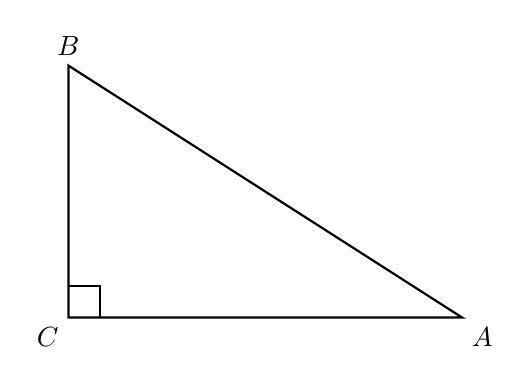
\begin{tikzpicture}
\coordinate (A) at (5,0);
\coordinate (B) at (0,3.2);
\coordinate (C) at (0,0);
\draw[thick] (A) -- (B) -- (C) -- cycle;
\draw[thick] (0.4,0) -- (0.4,0.4) -- (0,0.4);
\node[below left] at (C) {$C$};
\node[above] at (B) {$B$};
\node[below right] at (A) {$A$};
\end{tikzpicture}
\end{document}
